\section{Project time schedule}

We elected EGroupware for our project management matters which provides:
\begin{itemize}
 \item Time management
 \item Issue tracking
 \item Todo management and
 \item Cost tracking
\end{itemize}

\begin{landscape}
\begin{figure}[H]
 \centering
% 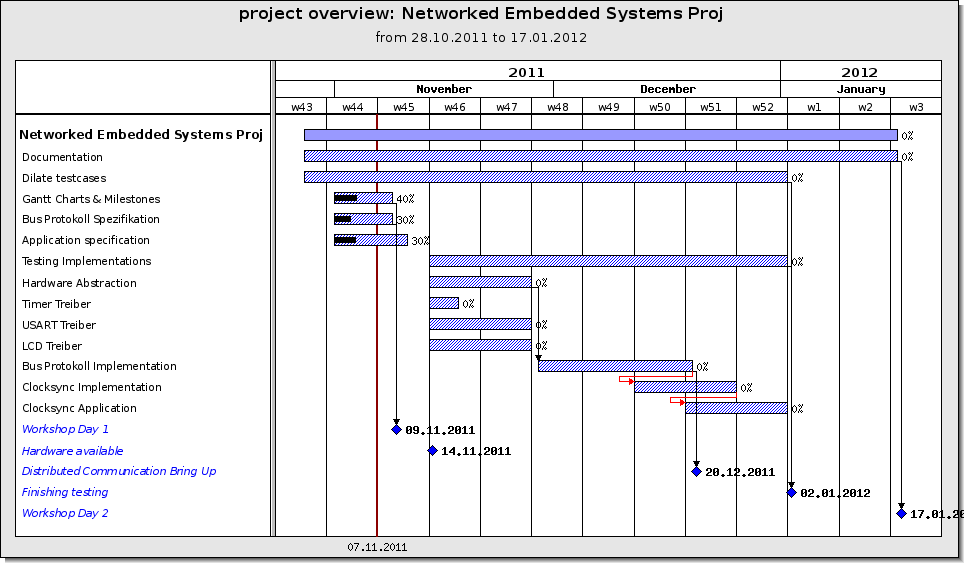
\includegraphics[angle=90,scale=0.6,keepaspectratio=true]{../images/201111_ganttchart.png}
 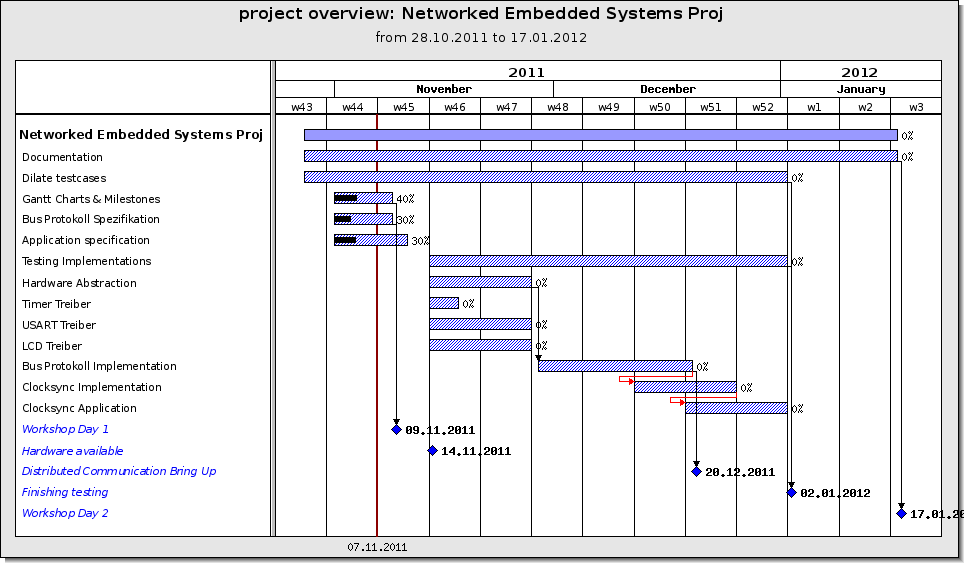
\includegraphics[scale=0.6,keepaspectratio=true]{../images/201111_ganttchart.png}
 % 201111_ganttchart.png: 964x563 pixel, 72dpi, 34.01x19.86 cm, bb=
 \caption{Gantt chart and time schedule}
 \label{fig:gantt chart}
\end{figure}
\end{landscape}

The gantt chart shown in figure \ref{fig:gantt chart} was exported from our project management tool and is described in the following sections.\\

\textbf{Legend:} \\
\begin{tabular}{lcl}
Start & ... & Planned starting date of the concerning task\\
End   & ... & Planned finishing date of the concerning task\\ 
Resources & ... & Expected resource consumption in percent\\
\end{tabular}


\subsection{Project presentation}
\begin{wrapfigure}{r}{0mm}
\begin{tabular}[t]{|lr|}
\hline
Start & kw43\\
End & kw46\\
Resources[\%] & 5\\
\hline
\end{tabular}
\end{wrapfigure}
Project presentation for the first workshop day.


\subsection{Documentation}
\begin{wrapfigure}{r}{0mm}
\begin{tabular}[t]{|lr|}
\hline
Start & kw43\\
End & kw3\\
Resources[\%] & 40\\
\hline
\end{tabular}
\end{wrapfigure}
Documentation is one of the main parts of project and refers to the entire project 
process flow and therefore lives over the entire project.\\
One of the main parts in this project is project management and we attach much 
importance to it and thus also on the documentation.\\

Documentation consists of: the documents \cite [NESD1]{NESD1} - \cite [NESD5]{NESD5} 
as well as in code documentation with doxygen.

\subsection{Dilate testcases}
\begin{wrapfigure}{r}{0mm}
\begin{tabular}[t]{|lr|}
\hline
Start & kw43\\
End & kw3\\
Resources [\%] & 10\\
\hline
\end{tabular}
\end{wrapfigure}
The matter of dialating testcases is to provide appropriate sets of conditions or variables under which
a tester is able to determine whether the application is working correctly or not.

Our test cases will include a description of the functionality to be tested and the preparation required
to ensure that the test can be conducted.\\
We will test our system in case of bus load and clock drifts so that we are able to get
significant test results to ensure our clocks can be synchronized in case of a high bus load.

\subsection{Gantt Charts \& Milestones}
\begin{wrapfigure}{r}{0mm}
\begin{tabular}[t]{|lr|}
\hline
Start & kw44\\
End & kw45\\
Resources [\%] & 5\\
\hline
\end{tabular}
\end{wrapfigure}
We are providing a Gantt Chart - that is a task dependent timeline - in form of a image output of our 
project management tool eGroupware. That includes milestones which are points 
in time bounded to the timelines in the Gantt Chart.
\subsection{Bus protocol specification}
\begin{wrapfigure}{r}{0mm}
\begin{tabular}[t]{|lr|}
\hline
Start & kw44\\
End & kw45\\
Resources [\%] & 10\\
\hline
\end{tabular}
\end{wrapfigure}
Our bus protocol specification provides a well structured communication interface and can be found in the document \cite [NESD2]{NESD2}.

It describes the operational purpose and the qualities of our bus protocol.
\subsection{Testing Implementations}
\begin{wrapfigure}{r}{0mm}
\begin{tabular}[t]{|lr|}
\hline
Start & kw46\\
End & kw52\\
Resources [\%] & 5\\
\hline
\end{tabular}
\end{wrapfigure}
Over the real process of implementation the hole team has to take care that their 
implementations are tested with the concerning testcase or with a miniature subset of a testcase.\\

Testing each implementation is an important part of the implementation an takes place during the implementation.

\subsection{Hardware Abstraction}
\begin{wrapfigure}{r}{0mm}
\begin{tabular}[t]{|lr|}
\hline
Start & kw46\\
End & kw48\\
Resources [\%] & 5\\
\hline
\end{tabular}
\end{wrapfigure}
Hardware abstraction includes the particular parts of concrete hardware APIs needed through the project. 
That means that the hardware abstraction layer (HAL) makes high level programming interfaces available to 
higher abstraction layers.

We broke down our main hardware parts to:
\begin{itemize}
 \item Timer driver\\
Which allows to initialize, set and get hardware timer concerning values that are needed
for further use regarding our bus communication, clock, clock synchronization and 
measurements concerning drift rates
 \item USART driver\\
Which allows us to arbitrate the bus and to send and receive data over the bus.
 \item LCD driver\\
Which allows us to initialize and draw text to the LC-Display.
\end{itemize}

\subsection{Bus Protocol Implementation}
\begin{wrapfigure}{r}{0mm}
\begin{tabular}[t]{|lr|}
\hline
Start & kw48\\
End & kw51\\
Resources [\%] & 10\\
\hline
\end{tabular}
\end{wrapfigure}
The bus protocol is the second main part of this project which includes the correct communication
between multiple nodes over the available bus connection. 
The bus itself is specified in \cite [NESD2]{NESD2} and deviations should stay small depending 
the protocol specification.
\subsection{Clock Synchronization Implementation}
\begin{wrapfigure}{r}{0mm}
\begin{tabular}[t]{|lr|}
\hline
Start & kw50\\
End & kw2\\
Resources [\%] & 10\\
\hline
\end{tabular}
\end{wrapfigure}
The clock synchronization and clocksync application is the third and last main part of 
this project where all conceived parts have to work together.

The bus will include a distributed clock while we will 
take a look at the following two synchronization methods
\begin{itemize}
 \item precision time protocol
 \item reference broadcast synchronization
\end{itemize}

\subsubsection{Clocksync Application}
The application is ment to:
\begin{itemize}
 \item measure drift rates through the clock sync processflow
 \item applying measurements in case of heavy bus load
\end{itemize}
